\documentclass[11pt, oneside]{article}   	% use "amsart" instead of "article" for AMSLaTeX format


% \usepackage{draftwatermark}
% \SetWatermarkText{Draft}
% \SetWatermarkScale{5}
% \SetWatermarkLightness {0.9} 
% \SetWatermarkColor[rgb]{0.7,0,0}


\usepackage{geometry}                		% See geometry.pdf to learn the layout options. There are lots.
\geometry{letterpaper}                   		% ... or a4paper or a5paper or ... 
%\geometry{landscape}                		% Activate for for rotated page geometry
%\usepackage[parfill]{parskip}    		% Activate to begin paragraphs with an empty line rather than an indent
\usepackage{graphicx}				% Use pdf, png, jpg, or eps� with pdflatex; use eps in DVI mode
								% TeX will automatically convert eps --> pdf in pdflat						
								% TeX will automatically convert eps --> pdf in pdflatex		
\usepackage{amssymb}
\usepackage{mathrsfs}
\usepackage{hyperref}
\usepackage{url}
\usepackage{subcaption}
\usepackage{authblk}
\usepackage{amsmath}
\usepackage{mathtools}
\usepackage{graphicx}
\usepackage[export]{adjustbox}
\usepackage{fixltx2e}
\usepackage{hyperref}
\usepackage{alltt}
\usepackage{color}
\usepackage[utf8]{inputenc}
\usepackage[english]{babel}
\usepackage{float}
\usepackage{bigints}
\usepackage{braket}
\usepackage{siunitx}

%
% so you can do e.g., \begin{bmatrix}[r] (or [c] or [l])
%

\makeatletter
\renewcommand*\env@matrix[1][c]{\hskip -\arraycolsep
  \let\@ifnextchar\new@ifnextchar
  \array{*\c@MaxMatrixCols #1}}
\makeatother

\newcommand{\argmax}{\operatornamewithlimits{argmax}}
\newcommand{\argmin}{\operatornamewithlimits{argmin}}

\title{A Few Notes on the Bloch Sphere}
\author{David Meyer \\ dmm@\{1-4-5.net,uoregon.edu\}}

\date{Last update: \today}							% Activate to display a given date or no date



\begin{document}
\maketitle

\section{Introduction}
\label{sec:intro}
The fundamental building block of classical computational devices is the two-state system. We typically think of these systems as being built from bits which can take values in $\{0,1\}$.
Quantum mechanics, on the other hand, tells us that any such system can exist in a superposition of states.  A \emph{qubit} is a quantum system in which the Boolean states $0$ and $1$
 are represented\footnote{I use Dirac or braket notion \cite{wang2007} in this document.}  by a prescribed pair of normalized and mutually orthogonal quantum states labeled as $\{\ket{0},\ket{1}\}$. 
 
 \bigskip
\noindent
More specifically, a qubit is defined as a 2-dimensional 
Hilbert space $H_2$ and we label an orthonormal basis of $H_2$ by $\{\ket{0}, \ket{1}\}$. The state of the qubit is an associated unit length vector in $H_2$. If a state is equal to a basis 
vector then we say it is a \emph{pure} state. If a state is any other linear combination of the basis vectors we say it is a \emph{mixed} state, or that the state is a superposition of 
$\ket{0}$ and $\ket{1}$. 

\bigskip
\noindent
The state of a qubit bit, $\ket{\psi}$,  is described by

\begin{equation*}
\ket{\psi}   = \alpha \ket{0} + \beta | \ket{1}
\end{equation*}

\bigskip
\noindent
where $\alpha, \beta \in \mathbb{C}$, $\ket{0} =  \begin{bmatrix} 1 \\ 0 \end{bmatrix}$, $\ket{1}  = \begin{bmatrix} 0 \\ 1 \end{bmatrix}$ and 
$|\alpha|^2 + |\beta|^2 = 1$.


\bigskip
\noindent
Here  $|x|^2 = xx^*$,  where  $x^*$ is the complex conjugate of $x$ \cite{wiki:complex_conjugate}. The complex plane is shown in
Figure \ref{fig:complex_plane_wiki}. Note: the Wikipedia uses "bar" ($\bar{x}$) to denote the complex conjugate as opposed to "star" ($x^*$).

\begin{figure}
\center{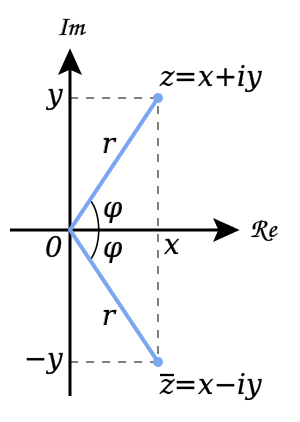
\includegraphics[scale=0.45] {images/complex_plane_wiki.png}}
\caption{The Complex Plane (Image courtesy Wikipedia \cite{wiki:complex_plane})}
\label{fig:complex_plane_wiki}
\end{figure}

\bigskip
\noindent
More generally, a \emph{quantum system} is an n-dimensional Hilbert Space $H_n$. We label an orthonormal basis on $H_n$
 by $\{\ket{x_1}, \ket{x_2}, \hdots, \ket{x_n}\}$ such that $x_i \in X$ for some finite $X$. The associated state of the system is a 
 unit length vector in $H_n$. If the state $S$ is  $\ket{\phi}$ at some moment in time, then we say that $S$ has state  $\ket{\phi}$
 or $S$ is in state  $\ket{\phi}$.
 
 \bigskip
 \noindent
 We can also see that a general form for the state of a quantum system is
 
 \begin{equation*}
 \sum\limits_{i = 1}^n \alpha_i \ket{x_i} \text{ where } \alpha_i \in \mathbb{C} \text{ and } \sum\limits_{i = 1}^n |\alpha_i|^2 = 1
 \end{equation*}

\bigskip
\noindent
\emph{Remark:}  We can already see an important technical problem that must be solved if quantum computers are ever to be practical. A superposition of states $\ket{0}$ and $\ket{1}$ is known 
as a \emph{coherent} state. A coherent state is extremely "unstable"; it inevitably interacts with its environment and collapses into a \emph{pure} state (see discussion below). This process is known as 
\emph{decoherence}. Algorithms that exploit quantum effects such as superposition are known as quantum algorithms. To apply 
these quantum algorithms in the real world, the \emph{decoherence time} must be longer than the time to run the algorithm. As a result methods for increasing the decoherence time 
are of great interest (see, for example \cite{2018PNAS..11510938L}).

\section{The Bloch Sphere}
One question that we might ask, given the complex plane representation of the state of a qubit, is "how does the real, 3-dimensional space in which we live correspond 
to the 2-dimensional representation of a qubit's state (as represented in the complex plane)"? The \emph{Bloch Sphere} gives us an elegant way to think about this question.

\begin{figure}[h]
\center{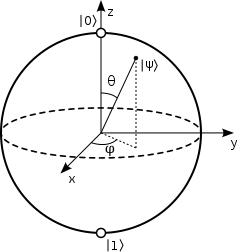
\includegraphics[scale=0.75] {images/bloch_sphere.png}}
\caption{The Bloch Sphere (Image courtesy Wikipedia \cite{wiki:bloch_sphere})}
\label{fig:bloch_sphere}
\end{figure}

\bigskip
\noindent
The Bloch Sphere, shown in Figure \ref{fig:bloch_sphere}, is named for the physicist Felix Bloch \cite{1946PhRv...70..460B} and gives us a beautiful way to think about and 
visualize the state of a qubit in 3-dimensional space.  

\bigskip
\noindent
In the Bloch Sphere the \emph{pure} state of a qubit $\ket{\psi}$  is represented as a point on the surface of the sphere. \emph{Mixed} states are represented
as points in the interior of the sphere.
Somewhat surprisingly, specification of a point on the Bloch Sphere requires only two parameters, 
$\theta$ and $\phi$. This itself is remarkable; you might imagine that describing a vector in 3-dimensional space might take three or more parameters. 

\bigskip
\noindent
The representation of a classical bits on the Bloch Sphere  is given by the poles of the sphere.  The representation of the probabilistic classical bit, that is, a bit that is $0$ with probability $p$ and $1$ with 
probability $1 - p$, is given by the point in z-axis with coordinate $2p - 1$. The interior of the Bloch Sphere is used to describe the states of a qubit in the presence of decoherence.

\bigskip
\noindent
The standard way to write the state of a qubit using the Bloch Sphere is 

\begin{equation}
\ket{\psi}  = \cos \frac{\theta}{2} \ket{0} + e^{i \phi} \sin \frac{\theta}{2} \ket{1}
\label{eqn:standard_psi}
\end{equation}

\bigskip
\noindent
where $0 \leq \theta \leq \pi$ and $0 \leq \phi \leq 2 \pi$. See Section \ref{subsec:derviing_equation_psi}  for a derivation of this equation. 

\subsection{Bloch Sphere Coordinate System}
Figure \ref{fig:bloch_sphere} shows the coordinate system of the Bloch Sphere.  Consider the $x$ axis. Here we can see that

\begin{flalign*}
& x_{+}:  \theta = \frac{\pi}{2}, \phi = 0  \longrightarrow \\
& \cos \frac{\pi}{4} \ket{0} + e^{i \cdot 0} \sin \frac{\pi}{4} \ket{1} \qquad  \qquad\qquad \mathrel{\#}  e^{i\cdot 0} = e^0 = 1 \\
&=  \frac{1}{\sqrt{2}} \ket{0} + (1)  \frac{1}{\sqrt{2}} \ket{1} \\
&=  \frac{1}{\sqrt{2}} \ket{0} + \frac{1}{\sqrt{2}} \ket{1} \qquad \qquad  \qquad\qquad \mathrel{\#}  H\ket{0} = \frac{1}{\sqrt{2}} \ket{0} + \frac{1}{\sqrt{2}} \ket{1} \\
& \equiv \ket{+} \\
\\
& x_{-}:  \theta = \frac{\pi}{2}, \phi = \pi \longrightarrow \\
& \cos \frac{\pi}{4} \ket{0} + e^{i  \pi} \sin \frac{\pi}{4} \ket{1} \qquad  \qquad\qquad \mathrel{\#}  \text{Euler's Identity  \cite{wiki:eulers_identity}: } e^{i\pi} + 1 = 0 , \;  e^{i\pi} = -1 \\
&=  \frac{1}{\sqrt{2}} \ket{0} + (-1)  \frac{1}{\sqrt{2}} \ket{1} \\
&=  \frac{1}{\sqrt{2}} \ket{0} -  \frac{1}{\sqrt{2}} \ket{1} \qquad \qquad  \qquad\qquad \mathrel{\#}  H\ket{1} = \frac{1}{\sqrt{2}} \ket{0} -  \frac{1}{\sqrt{2}} \ket{1} \\
& \equiv \ket{-} \\
\end{flalign*}

\noindent
On the $y$ axis of the Bloch Sphere  we can see that 


\begin{flalign*}
& y_{+}  :  \theta = \frac{\pi}{2}, \phi = \frac{\pi}{2} \longrightarrow \\
& \cos \frac{\pi}{4} \ket{0} + e^{i  \frac{\pi}{2}} \sin \frac{\pi}{4} \ket{1} 
\: \qquad \qquad \qquad\qquad \mathrel{\#}  \text{Euler's Formula  \cite{wiki:eulers_formula}: } e^{i\frac{\pi}{2}} = \cos \frac{\pi}{2} + i \sin  \frac{\pi}{2} = 0 + i \cdot 1 = i \\
&=  \frac{1}{\sqrt{2}} \ket{0} + i \frac{1}{\sqrt{2}} \ket{1} \\
&=  \frac{1}{\sqrt{2}} \ket{0} +  \frac{i}{\sqrt{2}} \ket{1} \\
\end{flalign*}

\begin{flalign*}
& y_{-} :  \theta = \frac{\pi}{2}, \phi = \frac{3 \pi}{2} \longrightarrow \\
& \cos \frac{\pi}{4} \ket{0} + e^{i  \frac{3 \pi}{2}}  \sin \frac{\pi}{4} \ket{1} 
\qquad \qquad \qquad\qquad \mathrel{\#}  e^{i\frac{3 \pi}{2}} = \cos \frac{3 \pi}{2}+ i \sin \frac{3 \pi}{2} = 0 - i \cdot 1 = -i \\
&=  \frac{1}{\sqrt{2}} \ket{0} - i \frac{1}{\sqrt{2}} \ket{1} \\
&=  \frac{1}{\sqrt{2}} \ket{0} -  \frac{i}{\sqrt{2}} \ket{1} 
\end{flalign*}

\bigskip
\noindent
Finally, on the $z$ axis of the Bloch Sphere  we can see that 


\begin{flalign*}
& z_{+}:  \theta = 0, \phi = 0 \longrightarrow \\
& \cos \frac{0}{2} \ket{0} + e^{i  0} \sin \frac{0}{2} \ket{1}  \\
&=  \cos 0 \ket{0} + (1)  \sin 0 \ket{1} \\
&=  1 \ket{0} + 0 \ket{1} \\
&= \ket{0} 
\end{flalign*}

\noindent
and

\begin{flalign*}
& z_{-}: \theta = \pi, \phi = 0 \longrightarrow \\
& \cos \frac{\pi}{2} \ket{0} + e^{i  0} \sin \frac{\pi}{2} \ket{1}  \\
&=  \cos 0 \ket{0} +  (1) \sin \frac{\pi}{2}  \ket{1} \\
&=  0 \ket{0} + 1 \ket{1} \\
&= \ket{1} 
\end{flalign*}


\bigskip
\noindent
So we can write the state of a qubit in many different ways. Perhaps the most generic way to write $\ket{\psi}$  is 

\begin{equation*}
\ket{\psi}  = \alpha \ket{0} + \beta \ket{1} 
\end{equation*}

\bigskip
\noindent
The maximally superimposed state is

\begin{equation}
\ket{\psi}  = \frac{1}{\sqrt{2}} \ket{0} + \frac{1}{\sqrt{2}} \ket{1} 
\label{eqn:entangled}
\end{equation}


\bigskip
\noindent
Here the probability of measuring $\ket{0}$ is $|a|^2 = aa^* = \Big ( \frac{1}{\sqrt{2}} \Big )^2 = \frac{1}{2}$.  Similarly,  and the probability of measuring $\ket{1}$ is $\frac{1}{2}$.  



\bigskip
\noindent
Now, note that 


\begin{equation}
\ket{\psi}  =  \frac{1}{\sqrt{2}} \ket{0} + \frac{1}{\sqrt{2}} \ket{1}  = \frac{1}{\sqrt{2}} \ket{0} + \frac{e^{i \theta}}{\sqrt{2}} \ket{1} 
\label{eqn:e_equality}
\end{equation}

\bigskip
\noindent
Why does the second equality in Equation \ref{eqn:e_equality} hold? In short its because $|\frac{e^{i \theta}}{\sqrt{2}} |^2 = |\frac{1}{\sqrt{2}}|^2$. But still why? 
Consider $|e^{i \theta}|^2$. By Euler's Formula\footnote{$e^{i\theta} = \cos \theta + i \sin \theta$} 

\begin{flalign*}
|e^{i\theta}|^2 &= |(\cos \theta + i \sin \theta )|^2 \\
&= (\cos \theta  + i \sin \theta )(\cos \theta  - i \sin \theta )  \\
&= \cos^2\theta  - \cos \theta  \; i \sin \theta  +  i \sin \theta  \cos \theta  - i^2 \sin^2 \theta  \\
&= \cos^2\theta  - i^2 \sin^2 \theta   \\
&= \cos^2\theta  +\sin^2 \theta   \\
&= 1
\end{flalign*}

\bigskip
\noindent
So $\ket{\psi}  = \frac{1}{\sqrt{2}} \ket{0} + \frac{1}{\sqrt{2}} \ket{1}  = \frac{1}{\sqrt{2}} \ket{0} + \frac{e^{i \theta}}{\sqrt{2}} \ket{1}$. 
This implies that the statistics of any measurements we could perform on the state $e^{i\theta} \ket{\psi}$ would be exactly the same 
as they would be for the state $\ket{\psi}$. This explains the claim in Section \ref{subsub:alpha_and_beta} that global phases 
have no physical significance. 


\bigskip
\noindent
We have seen that measuring $\ket{\psi}$ in the standard basis ($\{\ket{0}, \ket{1} \}$) yields a probability
of $\frac{1}{2}$ for measuring either $\ket{0}$ or $\ket{1}$. Is there any measurement that yields information about the phase $\theta$?

\bigskip
\noindent
Consider a measurement in a different basis, the $\{\ket{+},\ket{-}\}$ basis. As we saw above,  $\ket{+} \equiv \frac{1}{\sqrt{2}} (\ket{0} + \ket{1})$ and 
$\ket{-} \equiv \frac{1}{\sqrt{2}} (\ket{0} - \ket{1})$. What does $\ket{\psi}$ look like in this new basis? The basic approach is to first represent
$\ket{0}$ and $\ket{1}$ in the new basis. Here $\ket{0} =  \frac{1}{\sqrt{2}} (\ket{+} + \ket{-})$ and  $\ket{1} =  \frac{1}{\sqrt{2}} (\ket{+} - \ket{-})$. 
Then

\begin{flalign*}
\ket{\psi}  &= \frac{1}{\sqrt{2}} \ket{0} + \frac{e^{i \theta}}{\sqrt{2}} \ket{1} \\
&= \frac{1}{\sqrt{2}}  \Big (  \frac{1}{\sqrt{2}} \big (\ket{+} + \ket{-} \big) + \frac{e^{i \theta}}{\sqrt{2}} \big (\ket{+} -  \ket{-} \big) \Big ) \\
&= \frac{1}{2}  \big (\ket{+} + \ket{-} \big) +  \frac{e^{i \theta}}{2} \big ( \ket{+} -  \ket{-}  \big ) \\
&= \frac{1 + e^{i\theta}}{2}  \ket{+}  +  \frac{1- e^{i \theta}}{2} \ket{-} 
\end{flalign*}

\bigskip
\noindent
Since $e^{i\theta} = \cos \theta + i \sin \theta$  we can write

\begin{flalign*}
&=  \frac{ \big (1 + \cos \theta + i \sin \theta \big )}{2}  \ket{+}  +  \frac{ \big (1- (\cos \theta + i  \sin \theta  \big )\big )}{2} \ket{-} 
\end{flalign*}

\bigskip
\noindent
What then is the probability of measuring, say, $\ket{+}$, in the  $\{\ket{+},\ket{-}\}$ basis? Well, we know that the probability is the amplitude squared, so, 

\begin{flalign*}
P(\ket{+}) &=  \bigg | \frac{ \big (1 + \cos \theta + i \sin \theta \big )}{2} \bigg |^2 \\
&= \frac{1}{4} \big ((1 + \cos \theta + i \sin \theta) (1 + \cos \theta - i \sin \theta) \big ) \\
&= \frac{1}{4} \big (1 + \cos \theta - i \sin \theta + \cos \theta + \cos^2\theta - \cos \theta i \sin \theta + i \sin \theta + \cos \theta i \sin \theta - i^2 \sin^2 \theta \big ) \\
&= \frac{1}{4} \big (1 + 2 \cos \theta + \cos^2\theta + \sin^2 \theta \big )  \;  \qquad\qquad \mathrel{\#}  \cos^2 \theta + \sin^2 \theta = 1\\
&= \frac{1}{4} \big (1 + 2 \cos \theta + 1 \big ) \\
&= \frac{1}{4} \big (2 + 2 \cos \theta \big ) \\
&= \frac{1}{2} \big (1 + \cos \theta \big ) 
\; \qquad  \qquad \qquad \qquad \qquad\qquad \mathrel{\#} \cos \frac{\theta}{2} = \pm \sqrt{\frac{1 + \cos \theta}{2}}  \implies 1 + \cos \theta = 2 \cdot \cos^2 \frac{\theta}{2}\\
&= \frac{1}{2} \Big (2 \cdot \cos^2 \frac{\theta}{2} \Big ) \\
&= \cos^2 \frac{\theta}{2}  
\quad \qquad \qquad  \qquad \qquad \qquad \qquad\qquad \mathrel{\#} P(\ket{+}) =  \cos^2 \frac{\theta}{2}\\
\end{flalign*}

\noindent
Similarly, we know that the probability of measuring $\ket{-}$,  $P(\ket{-}) = \sin^2 \frac{\theta}{2}$.  So measuring the qubit in the $\{\ket{+},\ket{-}\}$ basis does reveal
some information about the phase $\theta$. More about this in Section \ref{subsec:derviing_equation_psi}.

\subsection{Why does $\theta$ vary between $0$ and $\pi$ in Equation \ref{eqn:standard_psi}?} 
\label{sec:later}
In the complex plane representation of $\ket{\psi}$, the basis vectors $\ket{0}$ and $\ket{1}$ are orthogonal, 
that is, there is a $\frac{\pi}{2}$ angle between them and hence their inner product $\braket{0|1} = 0$. In the Bloch Sphere the angle $\theta$ 
between $\ket{0}$ and $\ket{1}$ is  $\pi$. That is, in the Bloch Sphere $\ket{0}$ and  $\ket{1}$ are \emph{antipodal} rather than orthogonal.

\bigskip
\noindent
Further, in the general form of $\ket{\psi}$ (Equation \ref{eqn:ket_psi}),  $\alpha$ and $\beta$ are known as \emph{probability amplitudes} \cite{2013arXiv1304.5824K} 
and thus $0 \leq |\alpha| \leq 1$ (likewise for $\beta$). However, in the Bloch Sphere we have $0 \leq \theta \leq \pi$. So to keep the values of the probability 
amplitudes in the right range ($0 \leq |\alpha| \leq 1$) we need to divide $\theta$ by 2 (I'll just note here that there are many other ways to think about this).  
This is one reason that we see the angle $\frac{\theta}{2}$   in Equation \ref{eqn:standard_psi}. Having $\ket{0}$ and $\ket{1}$ represented on the same axis 
($z$) also saves a dimension in the Bloch Sphere representation. We will see further implications of $\ket{0}$ and $\ket{1}$ being antipodal rather than 
orthogonal in Section \ref{sec:normalization_constraint}.

\subsection{Deriving Equation \ref{eqn:standard_psi}}
\label{subsec:derviing_equation_psi}
Let's take a look at why Equation \ref{eqn:standard_psi} looks the way it does. First, remember that the general state of a qubit  is

\begin{equation}
\ket{\psi}  = \alpha \ket{0}  + \beta \ket{1}
\label{eqn:ket_psi}
\end{equation}

\bigskip
\noindent
where $\alpha, \beta \in \mathbb{C}$ and $\langle \psi | \psi \rangle = |\alpha|^2 + |\beta|^2 = 1$.  $|\alpha|^2 + |\beta|^2 = 1$ is known as a  \emph{normalization constraint}.
Here  $\langle \psi | \psi \rangle$ is the inner product of $\psi$ with itself, namely 
$\begin{bmatrix} \alpha & \beta \end{bmatrix} \begin{bmatrix} \alpha \\ \beta \end{bmatrix} = |\alpha|^2 + |\beta|^2$.
In general for two $n \times 1$ vectors \textbf{u} and \textbf{v},  the inner product  $\langle \mathbf{u} | \mathbf{v} \rangle$ is defined as

\begin{equation*}
\langle \mathbf{u} | \mathbf{v} \rangle = \mathbf{u}{^\text{T}}\mathbf{v}
\end{equation*}

\begin{figure}
\center{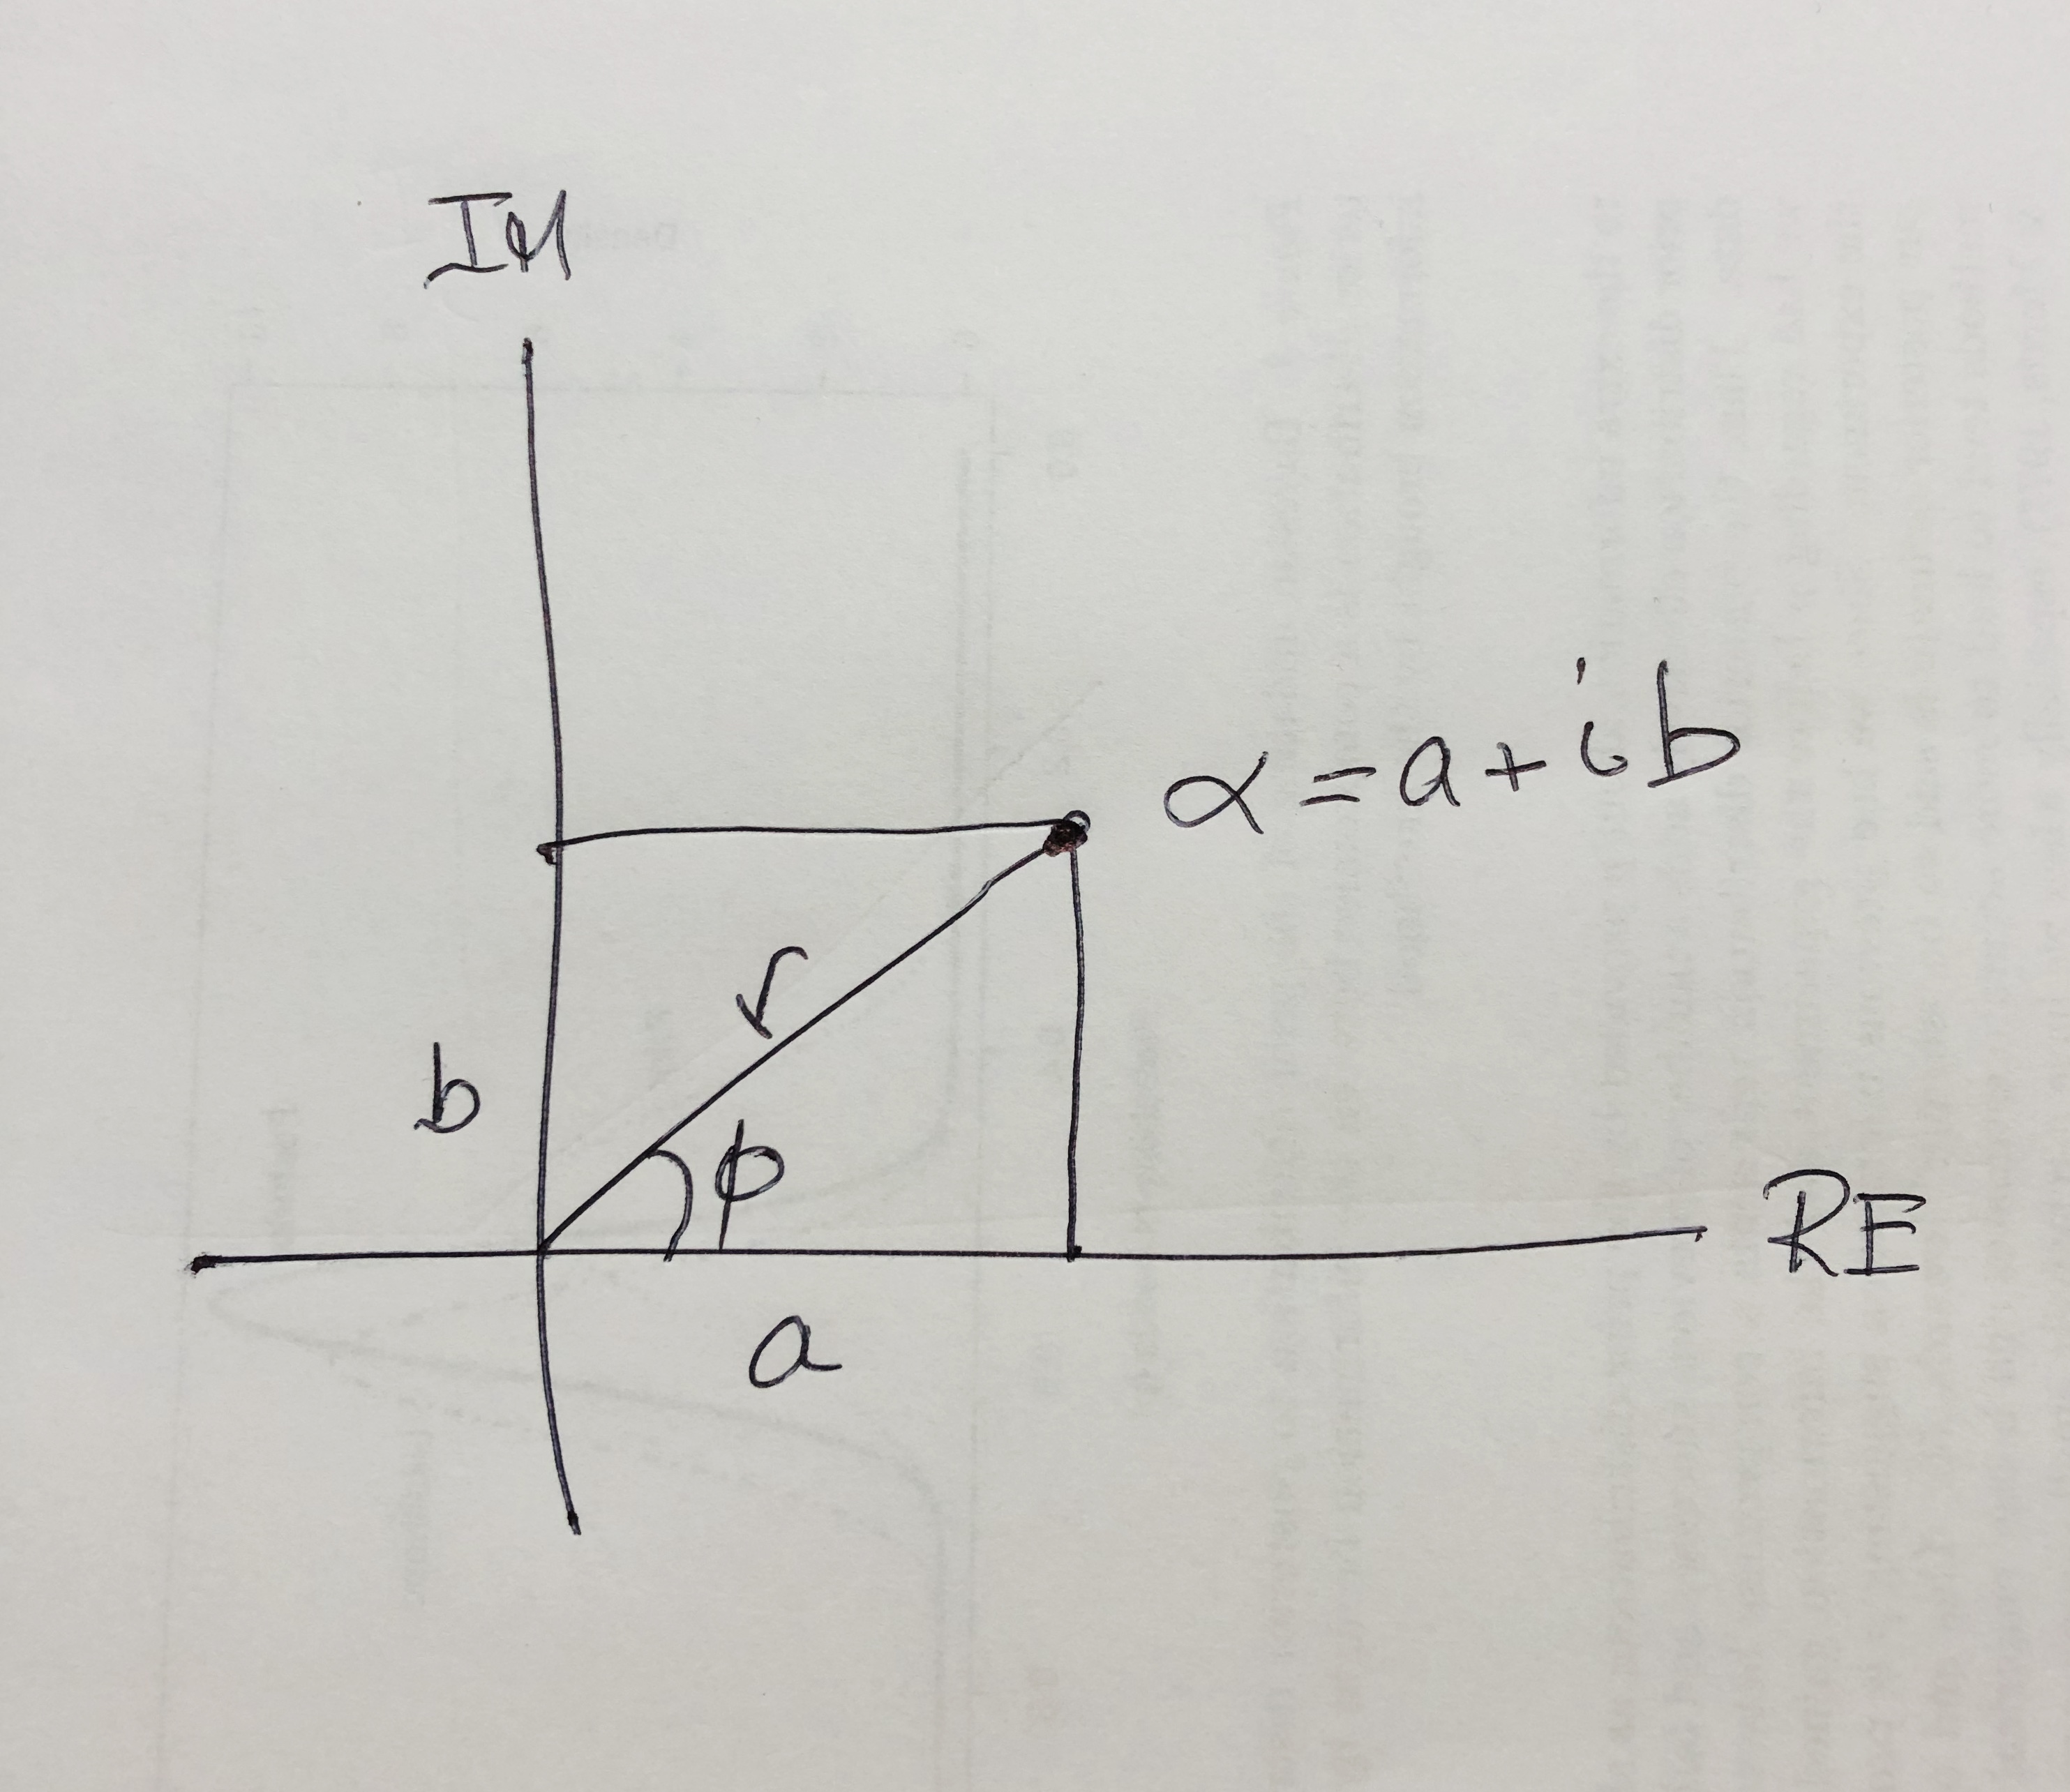
\includegraphics[scale=0.07, frame] {images/complex_plane_cartoon.jpg}}
\caption{$\alpha$ in the Complex Plane}
\label{fig:complex_plane_cartoon}
\end{figure}

\subsubsection{What can we say about $\alpha$ and $\beta$?}
\label{subsub:alpha_and_beta}
Since $\alpha$ and $\beta$ are complex numbers, we can write $\alpha$  (or $\beta$, with different $a$ and $b$) as  $\alpha = a + ib$. This is depicted
 in Figure \ref{fig:complex_plane_cartoon}.  There are a few things we can notice about $\alpha$. First, $a = r \cos \phi$; 
similarly, $b = r \sin \phi$. So we can write

\begin{flalign*}
\alpha &= a + ib \\
&= r \cos \phi+ i r \sin \phi \\
&=  r [\cos \phi +i \sin \phi]
\end{flalign*}

\noindent
Next we can apply Euler's Formula

\begin{flalign*}
\alpha &= a + ib 
\; \qquad \qquad\qquad\qquad \mathrel{\#} \alpha \text{ in the complex plane (Figure \ref{fig:complex_plane_cartoon})
} \\
&=  r [\cos \phi +i \sin \phi] 
\qquad\qquad \mathrel{\#} a = r \cos \phi, \:  b = r \sin \phi \text{, factor out } r\\
&= re^{i\phi} 
\, \quad \qquad\qquad \qquad\qquad \mathrel{\#} \text{Euler's Formula: }  e^{i\phi} = \cos \phi + i \sin \phi
\end{flalign*}

\bigskip
\noindent
So now let $\alpha = r_0e^{i\phi_0}$ and $\beta = r_1e^{i\phi_1}$. Then we have 

\begin{flalign*}
\ket{\psi}  &= \alpha \ket{0} + \beta \ket{1} = r_{0} e^{i \phi_0} \ket{0} + r_{1} e^{i \phi_1} \ket{1}
\end{flalign*}

\bigskip
\noindent
If we factor out $e^{i\phi_0}$, we get


\begin{equation*}
\ket{\psi} = e^{i \phi_0} [ r_{0} \ket{0} + r_{1} e^{i (\phi_1 - \phi_0)} \ket{1}]
\end{equation*}

\bigskip
\noindent
It turns out that the term $e^{i \phi_0}$, the global phase, has no physical significance \cite{2013arXiv1312.1463D}; 
you can rotate the axes any way you like with no effect so long as the x, y and z axes remain perpendicular to one another. So we 
can drop the $e^{i \phi_0}$  term and write


\begin{equation*}
\ket{\psi} = r_0 \ket{0} +  r_{1}e^{i (\phi_1 - \phi_0)} \ket{1}
\end{equation*}

\bigskip
\noindent
Next let $\phi = \phi_1 - \phi_0$. Then we have 


\begin{equation}
\ket{\psi} = r_{0} \ket{0} + r_{1} e^{i \phi} \ket{1}
\label{eqn:rket}
\end{equation}

\section{Normalization Constraints}
\label{sec:normalization_constraint}
One more observation we can make: Equation \ref{eqn:rket} tells us that 
we can write our normalization constraint $|\alpha|^2 + |\beta|^2 = 1$ as $|r_0|^2 + |r_{1}e^{i\phi}|^2 = 1$. 

\bigskip
\noindent
Since $r_0$ has no complex term $|r_0|^2 = r_0^2$ and we can write $r_0^2 + |r_{1}e^{i\phi}|^2 = 1$.  The term $|r_{1}e^{i\phi}|^2$ can be 
written as $r_{1}^2 |e^{i\phi}|^2$. So now we have $r_0^2 + r_{1}^2 |e^{i\phi}|^2  = 1$.

\bigskip
\noindent
But we can learn a bit more. Recall that $e^{i\phi} = \cos \phi + i \sin \phi$ (Euler's Formula), so  

\begin{flalign*}
|e^{i\phi}|^2 &= |(\cos \phi + i \sin \phi)|^2 \\
&= (\cos \phi + i \sin \phi)(\cos \phi - i \sin \phi)  \\
&= \cos^2\phi - \cos \phi \; i \sin \phi +  i \sin \phi \cos \phi - i^2 \sin^2 \phi \\
&= \cos^2\phi - i^2 \sin^2 \phi  \\
&= \cos^2\phi +\sin^2 \phi  \\
&= 1
\end{flalign*}


\noindent
The result is that the constraint $|\alpha|^2 + |\beta|^2 = 1$ can be written as $ r_0^2 + r_1^2 = 1$.
If we choose $r_0 = \cos x$ and $r_1 = \sin x$ then we'll have $\cos^2 x+ \sin^2 x= 1$ (by the Pythagorean 
trigonometric identity \cite{wiki:trig}),  which satisfies the normalization constraint. 

\bigskip
\noindent
If we now let $x = \frac{\theta}{2}$ (see Section \ref{sec:later}), 
we get Equation \ref{eqn:standard_psi}, namely  $\ket{\psi}  = \cos \frac{\theta}{2} \ket{0} + e^{i \phi} \sin \frac{\theta}{2} \ket{1}$.

\section{Qubits, Kronecker/Tensor Products and States}

If we consider two binary strings, say $011$ and $111$,  $011$ typically represents the (decimal) number $3$, while $111$ represents the number $7$. In general, three physical bits can be prepared in 
$2^3 = 8$ different configurations that can represent the integers from $0$ to $7$. However, a register composed of three classical bits can store only one number at a given moment of time. 
One of the powerful aspects of the quantum world is that a register composed of $3$ qubits can represent all $8$ configurations at the same time.

\bigskip
\noindent
As described in Section \ref{sec:intro}, a qubit is a quantum system in which the Boolean states $0$ and $1$ are represented by a pair of normalized and mutually orthogonal quantum 
states labeled as $\{\ket{0}, \ket{1}\}$.  These two states form a \emph{computational basis} and any other (pure) state of the qubit can be written as a superposition $\alpha \ket{0} + \beta \ket{1}$
for some $\alpha$ and $\beta$ such that $|\alpha|^2 + |\beta|^2 = 1$.  A collection of $n$ qubits is called a quantum register of size $n$.

\bigskip
\noindent
It is typically assumed that information is stored in the registers in binary form. For example, the number $6$ is represented by a register in state
$\ket{1} \otimes \ket{1} \otimes \ket{0}$.  In more compact notation: $\ket{a}$ stands for the tensor product 
$\ket{a_{n-1}}  \otimes \ket{a_{n - 2}} \otimes \cdots \otimes \ket{a_1} \otimes \ket{a_0}$,  where $a_i \in \{0,1\}$.
$\ket{a}$ represents a quantum register prepared with the value $a = 2^0a_0 + 2^1 a_1 + \cdots + 2^{n - 1}a_{n-1}$.
There are $2^n$ states of this kind, representing all binary strings of length $n$ or the numbers from 0 to $2^{n - 1}$ and form a convenient computational basis. Following 
convention, $a \in \{0, 1\}^n$ (a is a binary string of length $n$) implies that $\ket{a}$ belongs to the computational basis.

\subsection{Computational Basis}
The computational or standard basis of $\mathbb{C}^n$, denoted by $\{\ket{0}, \cdots, \ket{n - 1}\}$, is given by\footnote{Recall that 
$\begin{bmatrix} 
1 \\
\vdots \\
0
\end{bmatrix}$ 
is alternate notation for 
$\begin{pmatrix} 
1 \\
\vdots \\
0
\end{pmatrix}$.}

\begin{flalign*}
\ket{0} = 
\begin{bmatrix} 
1 \\
0 \\
\vdots \\
0
\end{bmatrix}, 
\ket{1} = 
\begin{bmatrix} 
0 \\
1 \\
\vdots \\
0
\end{bmatrix}, 
\hdots
\ket{n - 1} =
\begin{bmatrix} 
0 \\
0 \\
\vdots \\
1
\end{bmatrix}
\end{flalign*}

\bigskip
\noindent
Interestingly, the computational basis forms the set of \emph{one-hot} vectors such that $\ket{i}$ has a $1$ in the $i$th position and $0$ everywhere else.  The normalized sum of all computational 
basis vectors defines the vector

\begin{flalign*}
\ket{D} = \frac{1}{\sqrt{n}} \sum\limits_{i = 0}^{n - 1} \ket{i}
\end{flalign*}

\bigskip
\noindent
For a qubit, where $n = 2$, we have 

\begin{flalign*}
\ket{0} &= \begin{bmatrix} 1 \\ 0 \end{bmatrix} \\
\ket{1} &= \begin{bmatrix} 0 \\ 1 \end{bmatrix}  \\
\ket{D} &= \frac{1}{\sqrt{2}} \sum\limits_{i = 0}^{1} \ket{i}
\end{flalign*}

\noindent
As mentioned above, multiple qubits states can be prepared in a register. Typically the state of a register is represented by the tensor
product \cite{wiki:kronecker} of two or more qubit states. Let's take a quick look at how the tensor product works. 


\subsubsection{Tensor Products}

The Kronecker or tensor product, denoted by $\otimes$, is defined as follows: If
$\mathbf{A}$ is an $m \times n$ matrix and $\mathbf{B}$ is a $p \times q$ matrix, then the tensor product
$\mathbf{A} \otimes \mathbf{B}$ is the $mp \times nq$ block matrix

\bigskip
\begin{equation*}
\mathbf {A} \otimes \mathbf {B} =
\begin{bmatrix}a_{11}\mathbf {B} &\cdots &a_{1n}\mathbf {B} \\\vdots &\ddots &\vdots \\a_{m1}\mathbf {B} &\cdots &a_{mn}\mathbf {B} 
\end{bmatrix}
\end{equation*}

\bigskip
\noindent
For example \cite{wiki:kronecker}

\begin{equation*}
 \begin{bmatrix}
    1 & 2 \\
    3 & 4 \\
  \end{bmatrix}
\otimes
 \begin{bmatrix}
    0 & 5 \\
    6 & 7 \\
  \end{bmatrix} =
  \begin{bmatrix}
    1 \cdot \begin{bmatrix}
      0 & 5 \\
      6 & 7 \\
    \end{bmatrix} & 
    2 \cdot \begin{bmatrix}
      0 & 5 \\
      6 & 7 \\
    \end{bmatrix} \\

    3 \cdot \begin{bmatrix}
      0 & 5 \\
      6 & 7 \\
    \end{bmatrix} & 
    4 \cdot \begin{bmatrix}
      0 & 5 \\
      6 & 7 \\
    \end{bmatrix} \\
  \end{bmatrix} =
  \begin{bmatrix}
    1\cdot 0 & 1\cdot 5 & 2\cdot 0 & 2\cdot 5 \\
    1\cdot 6 & 1\cdot 7 & 2\cdot 6 & 2\cdot 7 \\
    3\cdot 0 & 3\cdot 5 & 4\cdot 0 & 4\cdot 5 \\
    3\cdot 6 & 3\cdot 7 & 4\cdot 6 & 4\cdot 7 \\
  \end{bmatrix} =
  \begin{bmatrix}
    0 & 5 & 0 & 10 \\
    6 & 7 & 12 & 14 \\
    0 & 15 & 0 & 20 \\
    18 & 21 & 24 & 28
  \end{bmatrix}
 \end{equation*}

\bigskip
\noindent
Consider the 3 qubit register $\ket{1} \otimes \ket{0} \otimes \ket{1} = \ket{101} = \ket{5}$. How does the tensor product 
$\ket{1} \otimes \ket{0} \otimes \ket{1}$ work here?

\begin{flalign*}
\ket{1} \otimes \ket{0} \otimes \ket{1} &= \ket{1}  \otimes \begin{bmatrix} 1 \\ 0 \end{bmatrix} \otimes  \begin{bmatrix} 0 \\ 1 \end{bmatrix} \\
&= \ket{1} \otimes 
\begin{bmatrix}
1 \cdot  \begin{bmatrix} 0 \\ 1\end{bmatrix} \\
0 \cdot \begin{bmatrix} 0 \\ 1\end{bmatrix} 
\end{bmatrix} \\
&=
\ket{1} \otimes 
\begin{bmatrix}
 0 \\ 1 \\ 0 \\ 0
\end{bmatrix} \\
&= 
\begin{bmatrix} 0 \\ 1\end{bmatrix}
\otimes
\begin{bmatrix}
 0 \\ 1 \\ 0 \\ 0
\end{bmatrix} \\
&=
\begin{bmatrix}
0 \cdot  \begin{bmatrix}
 0 \\ 1 \\ 0 \\ 0
\end{bmatrix} \\
1 \cdot  \begin{bmatrix}
 0 \\ 1 \\ 0 \\ 0
\end{bmatrix}
\end{bmatrix} \\
&= 
\begin{bmatrix}
0 \\ 0 \\ 0 \\  0 \\
0 \\  1  \\  0 \\ 0
\end{bmatrix} \\
&= \begin{bmatrix} 0 & 0 & 0 &  0 & 0 &  1 &  0 & 0 \end{bmatrix}^{\text{T}}\\
& = \ket{101} \\
&= \ket{5}
\end{flalign*}

\bigskip
\noindent
Notice that the vector  $\begin{bmatrix} 0 & 0 & 0 &  0 & 0 &  1 &  0 & 0 \end{bmatrix}^{\text{T}}$ is of length $2^3$ and is the one-hot encoding of $\ket{101}$.

\subsection{Superpositions}
A classical register of size three, like a quantum register of size three, can store one of $2^3$ numbers such as $3$ or $7$, as follows

\begin{flalign*}
\ket{0} \otimes \ket{1} \otimes \ket{1} &\equiv \ket{011} \equiv \ket{3} \\
\ket{1} \otimes \ket{1} \otimes \ket{1} &\equiv \ket{111} \equiv \ket{7}
\end{flalign*}

\bigskip
\noindent
However, unlike a classical register, a quantum register can be prepared in the superposition of some or all of its qubits.  For example, if instead of setting the first qubit to 
$\ket{0}$ or $\ket{1}$, we prepare it in the superposition $\frac{1}{\sqrt{2}} (\ket{0} + \ket{1})$, then we have

\begin{flalign}
\label{eqn:super}
\frac{1}{\sqrt{2}} (\ket{0} + \ket{1})  \otimes \ket{1} \otimes \ket{1} \equiv \frac{1}{\sqrt{2}} (\ket{011} + \ket{111})  \equiv \frac{1}{\sqrt{2}} (\ket{3} + \ket{7}) 
\end{flalign}

\bigskip
\noindent
There is nothing special about Equation \ref{eqn:super}. We can also prepare a 3 qubit register in a superposition of all eight states by putting 
each qubit into the superposition $\frac{1}{\sqrt{2}} (\ket{0} + \ket{1})$. This gives us

\begin{flalign*}
\frac{1}{\sqrt{2}} (\ket{0} + \ket{1}) \otimes \frac{1}{\sqrt{2}} (\ket{0} + \ket{1}) \otimes \frac{1}{\sqrt{2}} (\ket{0} + \ket{1})
\end{flalign*}

\noindent
which can also be written as 

\begin{flalign*}
2^{- \frac{3}{2}} \Big (\ket{000} + \ket{001} + \ket{010} + \ket{011} + \ket{100}+ \ket{101} + \ket{110} + \ket{111} \Big)
\end{flalign*}

\noindent
or in decimal
\begin{flalign*}
2^{- \frac{3}{2}} \Big  (\ket{0} + \ket{1} + \ket{2} + \ket{3} + \ket{4}+ \ket{5} + \ket{6} + \ket{7} \Big) = 
2^{- \frac{3}{2}}  \sum\limits_{i = 0}^{7} \ket{i}
\end{flalign*}

\bigskip
\noindent
This kind of qubit preparationn and any other manipulation of qubits must be performed by unitary operator (matrix)\footnote{Recall that a unitary matrix $U$ has the property that
$UU^\dagger = U^{\dagger}U= I$, where $U^\dagger$ is the conjugate transpose, or \emph{adjoint}, of $U$ and $I$ is the identity matrix \cite{wiki:unitary_matrix}.}. A quantum logic gate is a device 
which performs a fixed unitary operation on selected qubits in a fixed period of time and a quantum network is a device consisting of quantum logic gates whose computational 
steps are synchronized in time \cite{PhysRevA.54.147}.


\bigskip
\noindent
This is kind of interesting: The \emph{Hadamard} transform (or gate) \cite{wiki:hadamard}, $H$, defined as

\begin{flalign*}
H = \frac{1}{\sqrt{2}}  \begin{bmatrix}[r] 1 & 1 \\ 1 &  -1 \end{bmatrix}
\end{flalign*}

\bigskip
\noindent
transforms $\begin{bmatrix}[r] 1 \\  0 \end{bmatrix}$ into  $\frac{1}{\sqrt{2}} \begin{bmatrix} 1 \\  1 \end{bmatrix}$. That is,  $H \ket{0} = \frac{1}{\sqrt{2}} (\ket{0} + \ket{1})$. This is also called
the $\ket{+}$ state. Similarily,
$H \ket{1} = \frac{1}{\sqrt{2}} (\ket{0} -  \ket{1}) \equiv \ket{-}$.

\bigskip
\noindent
Now, what is the value of $H (H \ket{0})$?  First, observe that 

\begin{flalign*}
H \ket{0} &= \frac{1}{\sqrt{2}} \begin{bmatrix}[r] 1 & 1 \\ 1 & -1 \end{bmatrix}  \begin{bmatrix}1 \\  0  \end{bmatrix} = 
\frac{1}{\sqrt{2}}  \begin{bmatrix}[l] 1 \cdot 1 + 1 \cdot 0 \\  1 \cdot 1 + -1 \cdot 0 \end{bmatrix}  =
\frac{1}{\sqrt{2}} \begin{bmatrix} 1 \\ 1\end{bmatrix} 
\qquad \qquad \mathrel{\#}  H \ket{0}  = \frac{1}{\sqrt{2}} (\ket{0} + \ket{1})
\end{flalign*}

\bigskip
\noindent
Here's an interesting observation. It turns out that the positive and negative amplitudes 
of $\ket{1}$ in $H (H \ket{0})$ cancel out.  This effect is called \emph{interference}, and is analogous to interference patterns between light or sound waves.
So why is this?

\begin{flalign*}
H(H \ket{0})  &= \frac{1}{\sqrt{2}} \begin{bmatrix}[r]1 & 1 \\ 1 & -1 \end{bmatrix} \Bigg ( \frac{1}{\sqrt{2}}  \begin{bmatrix}1 \\  1  \end{bmatrix} \Bigg ) \\
&= \frac{1}{2}  \begin{bmatrix}[r]1 & 1 \\ 1 & -1 \end{bmatrix}  \begin{bmatrix}1 \\  1  \end{bmatrix}  \\
&= \frac{1}{2} \begin{bmatrix}[l]1 \cdot 1 + 1 \cdot 1 \\ 1 \cdot 1 + -1 \cdot 1 \end{bmatrix} \\
&= \frac{1}{2} \begin{bmatrix} 2 \\ 0 \end{bmatrix} \\
&= \begin{bmatrix}  \frac{1}{2} \cdot 2 \\  \frac{1}{2} \cdot 0 \end{bmatrix} \\
& = \begin{bmatrix} 1 \\ 0 \end{bmatrix} \\
&= \ket{0}
\end{flalign*}

\bigskip
\noindent
Now, if we apply the Hadamard gate $H$ to each bit of a $n$ bit register containing all zeros, we get the superposition of all $n$-bit strings, namely

\begin{equation*}
\frac{1}{\sqrt{2^n}} \sum\limits_{j \in \{0,1\}^n} \ket{j}
\end{equation*}

\bigskip
\noindent
More generally, if we apply $H^{\otimes n}$ to an initial state $\ket{i}$ with $i \in \{0,1\}^n$ we get the $n$-fold Hadamard transform, denoted  $H^{\otimes n} \ket{i}$ and 
defined as follows

\begin{equation*}
H^{\otimes n} \ket{i} = \frac{1}{\sqrt{2^n}} \sum\limits_{j \in \{0,1\}^n} (-1)^{i \cdot j} \ket{j}
\end{equation*}

\noindent
where $i \cdot j = \sum\limits_{k = 1}^n i_{ k}j_{k}$ is the inner product of the $n$-bit strings $i,j \in \{0,1\}^n$. For example
\begin{flalign*}
H^{\otimes 2} \ket{01} &=  H \ket{0} \otimes H \ket{1} 
\; \qquad  \qquad \qquad \qquad \mathrel{\#} H^{\otimes 2} \ket{01} = H \ket{0} \otimes H  \ket{1}  = \ket{+} \otimes \ket{-} =  \ket{\uparrow} \otimes \ket{\downarrow} \\
&= \frac{1}{\sqrt{2}} (\ket{0} + \ket{1}) \otimes  \frac{1}{\sqrt{2}}  (\ket{0} - \ket{1}) 
\quad \mathrel{\#}  H = H^{\otimes 1} \\
&= \frac{1}{2} \big ( \ket{00} - \ket{01} + \ket{10} - \ket{11} \big ) \\
&= \frac{1}{2} \sum\limits_{j \in \{0,1\}^2} (-1)^{01 \cdot j} \ket{j}
\end{flalign*}

\section{Acknowledgements}

\newpage
\bibliographystyle{plain}
\bibliography{/Users/dmm/papers/bib/qc}
\end{document} 
